\section{Literature review}


这篇文献综述探讨了生物组织切片中技术的融合,特别关注图像分类和深度学习在优化切片参数方面的应用。它旨在突出重要的进展,确定当前方法学中存在的差距,并为拟议的项目奠定基础。

\subsection{切片机与显微镜}

近年来,自动切片机的出现显著简化了切片过程,并提高了切片的质量。

Zimmermann在文章"Improved reproducibility in preparing precision-cut liver tissue slices"中,主张使用新的Leica振动刀来提高大鼠、小鼠和人体组织切片的精度和重复性 \cite{LR.1}。

在这个实验中,我们使用Epredia提供的HM355S切片机进行切片。这台机器是生物组织切片研究的流行设备,许多实验和论文都使用了这台设备进行切片。

Elzbieta Klimuszko使用HM355S切片机切割牙齿,以研究牙釉质中的钙和镁含量 \cite{LR.2}。

Andelko Hrzenjak也使用HM355S切片机切割病理性子宫内膜组织,以研究子宫内膜癌发展的机制 \cite{LR.3}。

同样,显微镜的选择也至关重要。在这个实验中,我们使用Keyence的VHX7000显微镜进行图像采集。它能够捕获生物组织切片的图像(例如,小鼠前列腺细胞 \cite{LR.4}),以及无机材料(如陶瓷 \cite{LR.5},玻璃 \cite{LR.6})。

实验将使用HM355s切片机和VHX7000显微镜进行切片和图像采集。这种设置确保了设备选择和技术应用的最佳配合,以提高组织切片过程的精度和效率,支持研究项目的总体目标。

% \subsection{深度学习的原理}







\subsection{医学图像分类-基于卷积神经网络}

对于医学图像分类问题来说,以卷积神经网络为主的深度学习模型已经被证实是最有效的方法之一。\cite{5.1 1}

卷积神经网络(CNN)是一种深度学习模型,尤其擅长处理图像数据。它通过一系列卷积层自动学习空间层次的特征,无需手动特征提取。一个典型的CNN模型包括卷积层、池化层、全连接层等\cite{DL.4}。一个典型的CNN架构如下所示:\cite{4.30 1}


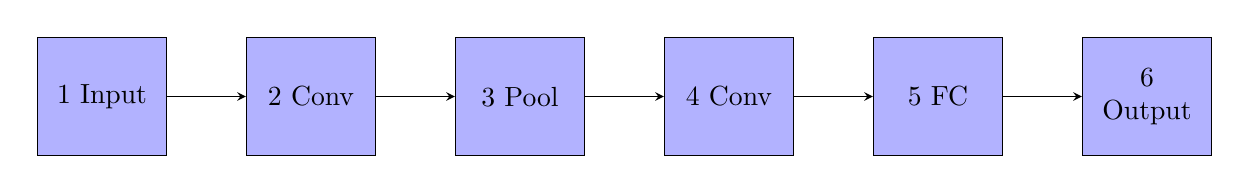
\begin{tikzpicture}[
    node distance=1cm and 0.5cm,
    block/.style={rectangle, draw, text width=4em, text centered, minimum height=15mm, fill=blue!30},
    arrow/.style={->,>=stealth}
]

% Define nodes in a matrix
\matrix [column sep=10mm, row sep=10mm] {
  \node (n1) [block] {1 Input}; & \node (n2) [block] {2 Conv}; & \node (n3) [block] {3 Pool} ;& \node
  (n4) [block] {4 Conv};    & \node (n5) [block] {5 FC};   & \node (n6) [block] {6 Output}; \\
};

% Connect nodes
\draw [arrow] (n1) -- (n2);
\draw [arrow] (n2) -- (n3);
\draw [arrow] (n3) -- (n4);
\draw [arrow] (n4) -- (n5);
\draw [arrow] (n5) -- (n6);
\end{tikzpicture}

在这个模型中:

\textbf{卷积层(Conv)}:这是CNN的核心层,负责从图像中提取特征。

\textbf{池化层(Pool)}:这些层用于减少特征图的维度,从而降低计算负载。

\textbf{全连接层(FC)}:这些层整合了卷积层和池化层提取的特征,用于分类或回归分析,最终导致输出。

对于一个典型的训练CNN的方法,包括前向传播、损失计算、反向传播和权重更新的过程。\cite{4.30 2}
\begin{enumerate}
    \item 前向传播:输入数据通过网络的每一层,直到输出层。
    \item 计算损失:使用损失函数(如交叉熵损失)计算网络输出和实际标签之间的差异。
    \item 反向传播:计算损失函数关于网络权重的梯度。
    \item 权重更新:使用梯度下降算法或其变种(如Adam或RMSprop)来更新网络权重,目标是减少损失函数的值。
\end{enumerate}
一旦训练完成,CNN可以用来预测新的、未见过的图像的标签。CNN的独特之处在于它们能够自动且高效地学习不同层次的抽象特征,使它们对于涉及复杂图像数据的任务非常有效,如医学图像分析,其中准确性和细节至关重要。\cite{4.30 3}

\subsection{医学图像分类-基于迁移学习}

对于CNN模型来说,一个显而易见的提升深度学习性能的方法是迁移学习。Sudhakar指出,在面对复杂分类问题比如恶意软件分类问题时,拥有大量参数的深度学习模型性能会显著优于传统机器学习模型。然而,由于深度学习模型需要大量的数据和计算资源,迁移学习成为了一个重要的解决方案。\cite{5.1 2}

迁移学习是一种机器学习方法,通过将一个模型训练的知识迁移到另一个模型上,从而加速训练过程。迁移学习的核心思想是利用源领域的知识来帮助目标领域的学习。\cite{4.30 4}

对于CNN模型,有几种迁移学习的方法,如微调和特征提取:

\textbf{微调}涉及调整预训练模型的参数以适应新任务。这通常包括在新数据上重新训练一些卷积层和全连接层,使模型能够将特征微调到新数据集的特定特性。\cite{4.30 5}

\textbf{特征提取}涉及使用预训练模型作为固定的特征提取器,其中只有全连接层在新数据上进行训练。在这种方法中,卷积层保持其学习的权重,并仅用于提取特征,这些特征然后被新训练的分类器层用于执行特定于新数据集的任务。\cite{4.30 6}

在Kora的研究中\cite{5.1 3},迁移学习能够消除从头开始训练模型的需要,并且能够在保证医学切片识别准确率的情况下,需要更少的数据。这种方法在医学图像分类问题中具有广泛的应用前景。

\subsection{关于切片组织的深度学习}

在生物医学领域,深度学习技术的应用已取得了显著的进步。深度学习模型在图像分类、对象检测和分割等任务中表现出色,为生物医学实验室的研究和诊断提供了强大的工具。

Lorena Guachi-Guachi 提出了一种利用 CNN 网络识别和精炼组织切片的方法。这种方法代表了深度学习的创新应用,可以提高组织准备和分析的精度 \cite{LR.7}。

在《生物医学纹理分析》一书中,Vincent Andrearczyk 介绍了一种专为纹理分析设计的 CNN 架构,与传统架构相比,这种架构显著提高了生物组织分类的准确性 \cite{LR.8}。这一发展展示了深度学习提高组织特性详细分析的潜力,这对于准确的诊断和研究至关重要。

Yan Xu 提出,从在大型自然图像数据库 ImageNet 上训练的 CNN 中提取的特征可以转移到组织的病理学图像上 \cite{LR.9}。这为实施转移学习提供了一种可行的方法,可以大大提高组织图像分类和分析的效率。

根据文献,深度学习技术在组织切片的图像分类和分析中有广阔的应用前景。通过利用深度学习模型,可以实现组织样本的有效识别和分类,为优化切片参数提供了强大的支持。

这一部分强调了深度学习对组织切片领域的变革性影响,预示着在组织学分析的准确性和实用性方面的显著改进。

\FloatBarrier % Now figures cannot float above section title
